\section{Five Two-Factor Authentication Methods}

\subsection{SMS}
\begin{frame}
  \frametitle{\currentsectionname}
  \begin{itemize}
    \item Confirmation code is sent as an SMS message
    \item Input of code into app
    \item Most widely used
    \item Some usability and security issues, but simple setup
  \end{itemize}
  \note{
    Usability Problems:
    \begin{itemize}
      \item delayed or no delivery
      \item user error when entering code
    \end{itemize}
    Security Problems:
    \begin{itemize}
      \item no encryption \textrightarrow{} Man In The Middle Attack
      \item SIM-Swapping \textrightarrow{} way to steal phone number, so codes are sent to wrong user
      \item Brute-Force attacks are possible, since codes are quite short
    \end{itemize}
  }
\end{frame}

\subsection{TOTP}
\begin{frame}
  \frametitle{\currentsectionname}
  \begin{itemize}
    \item \textit{Time-based One-time Password}
    \item User scans QR code, scanner generates confirmation code
    \item Confirmation code is entered and verified by server
    \item Code has limited lifespan
    \item Special scanner or smartphone required
  \end{itemize}

  \note{
    \begin{itemize}
      \item requires no internet access or phone reception\textrightarrow{} less attack surface
    \end{itemize}
    Usability Problems:
    \begin{itemize}
      \item relatively complicated to setup
      \item user error when entering code
    \end{itemize}
    Security:
    \begin{itemize}
      \item Encrypted \textrightarrow{} better than SMS
    \end{itemize}
  }
\end{frame}

\subsection{Pre-Generated Codes}
\begin{frame}
  \frametitle{\currentsectionname}
  \begin{itemize}
    \item List of codes is pre-generated
    \item Approximately eight characters long
    \item Codes must be stored securely
  \end{itemize}

  \note{
    \begin{itemize}
      \item relatively long codes may lead to errors when storing or entering them
      \item Users need to store codes securely, can be stolen
      \item codes valid for a long time \textrightarrow{} brute force possible
    \end{itemize}
  }
\end{frame}

\subsection{Push Notifications}
\begin{frame}
  \frametitle{\currentsectionname}
  \begin{enumerate}
    \item User receives notification on smartphone
    \item Option to confirm or deny login attempt
  \end{enumerate}
  \begin{itemize}
    \item Requires smartphone and typically specific app
    \item No input of code required
    \item Fast and convenient
  \end{itemize}

  \note{
    \begin{itemize}
      \item notification needs to be sent to right device \rightarrow{} ideally the device nearest to the user
      \item no need to enter code \textrightarrow{} less prone to error
    \end{itemize}
  }
\end{frame}

\subsection{U2F Security Tokens}
\begin{frame}
  \frametitle{\currentsectionname}
  \begin{columns}
    \begin{column}{0.7\textwidth}
      \begin{itemize}
        \item \textit{Universal 2nd Factor}
        \item User uses a U2F-compatible hardware device, such as a security key, to authenticate
        \item Fast and secure
        \item Requires U2F hardware device
      \end{itemize}
    \end{column}
    \begin{column}{0.3\textwidth}
      \begin{figure}
        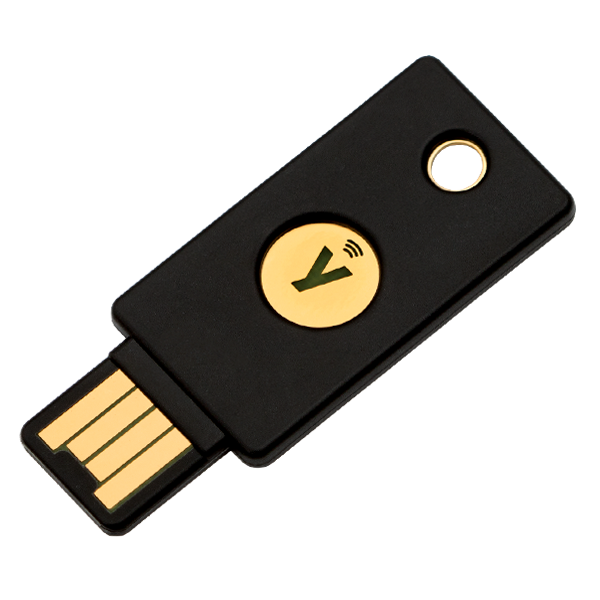
\includegraphics[height=\linewidth]{ubikey}
        \caption{YubiKey\endnote{\url{https://media.yubico.com/media/catalog/product/5/n/5nfc_hero_2021.png}}}
      \end{figure}
    \end{column}
  \end{columns}

  \note{
    \begin{itemize}
      \item conceived as a very secure, but still usable method
            \begin{itemize}
              \item[\textrightarrow] that's why very interesting later, when we look at the study results
            \end{itemize}
      \item Security Risk: Loss of U2F token
            \begin{itemize}
              \item[\textrightarrow] important to have a backup safely stored away
            \end{itemize}
    \end{itemize}
  }
\end{frame}
